
\section*{Dice \& Tests}



\begin{eptable}{ l | X }
   \epheader{2}{Success Result}
    $Success\,\geq\,33 $ & Superior success.\\
    $Success\,\geq\,66$ & 2x Superior success.\\
    $Failure\,\leq\,66$ & Superior failure.\\
    $Failure\,\leq\,33$ & 2x Superior failure.\\
    00, \num{11}, \ldots \num{99} & Critical. Supersedes superior. 00 always success / \num{99} failure.\\
\end{eptable}

$Success\,\geq\,33$ means the player rolled a success
\textit{and} also rolled higher than \num{33}.


\bigskip

\begin{eptable}{ l | X }
   \epheader{2}{Superiors}
    Quality &  Work more exact or more sloppy. Subsequent tests maybe $\pm\,10$.\\
    Quantity & Consumes or produces fewer or more materials or results.\\
    Detail & Acquire information in more or less detail / depth.\\
    Time & Task takes shorter or longer time $\pm\,25\%$ Task action only.\\
    Covertness & Action more or less obvious or attention drawing, $\pm\,10$.\\
    Damage & Success only. Inflict \dv{1d6} more.\\
\end{eptable}

Players can chose two effects, or same effect twice on double superior.

\bigskip


\begin{eptable}{ X }
   \epheader{1}{Criticals}
   Double damage on attack. \\
   Gain $\pm\,20$ on next test. \\
   Take (success) or lose (failure) next action. \\
   Break weapon or tool (failure). \\
   % Regain \num{1} Insight, Moxie, Vigor (success). \\
   Any other appropriate \textit{wow!} moment.\\
\end{eptable}

As always, the GM is encouraged to be creative.

\bigskip
%\subsection*{Additional Rules}

\begin{itemize}
 \itembox Always round true ($9/2=5$)
 \itembox Defaulting (using aptitude only), may imply additional \modifier{-10} to \modifier{-30}.
 \itembox Teamwork (all do the same in parallel): only \textbf{one} person rolls.
 \itembox Teamwork (constructively helping): highest person rolls,
         \modifier{+10} per helping character with useful aptitude over \num{40}.
\end{itemize}

\subsection*{Types of Tests}



\begin{eptable}{ l | X }
   \epheader{2}{Tests \& Actions}
    Success Test & Regular test as described above.\\
    Opposed Test & Highest succeeding roll wins. Critical trumps higher. \\
    Task Action & Roll at start. Failure apparent after \SI{25}{\percent} ($+\,25\%$ per sup. fail). \\
    Taking Time & Per \SI{25}{\percent} longer, get \modifier{+10} to test, max \modifier{+60}. At least 1 min.\\
    Rushing & Per \SI{25}{\percent} shorter, get \modifier{-20} to test, max \modifier{-60}.\\
\end{eptable}


\begin{itemize}
 \itembox Trying again induces cumulative \num{-10} modifier. GM may decide trying again not possible.
\end{itemize}


\begin{figure}[htb!]%
   \centering
   
\includegraphics[scale=0.95]{gfx/dice-modifiers}%
\end{figure}%

\begin{figure}[htb!]%
   \centering
   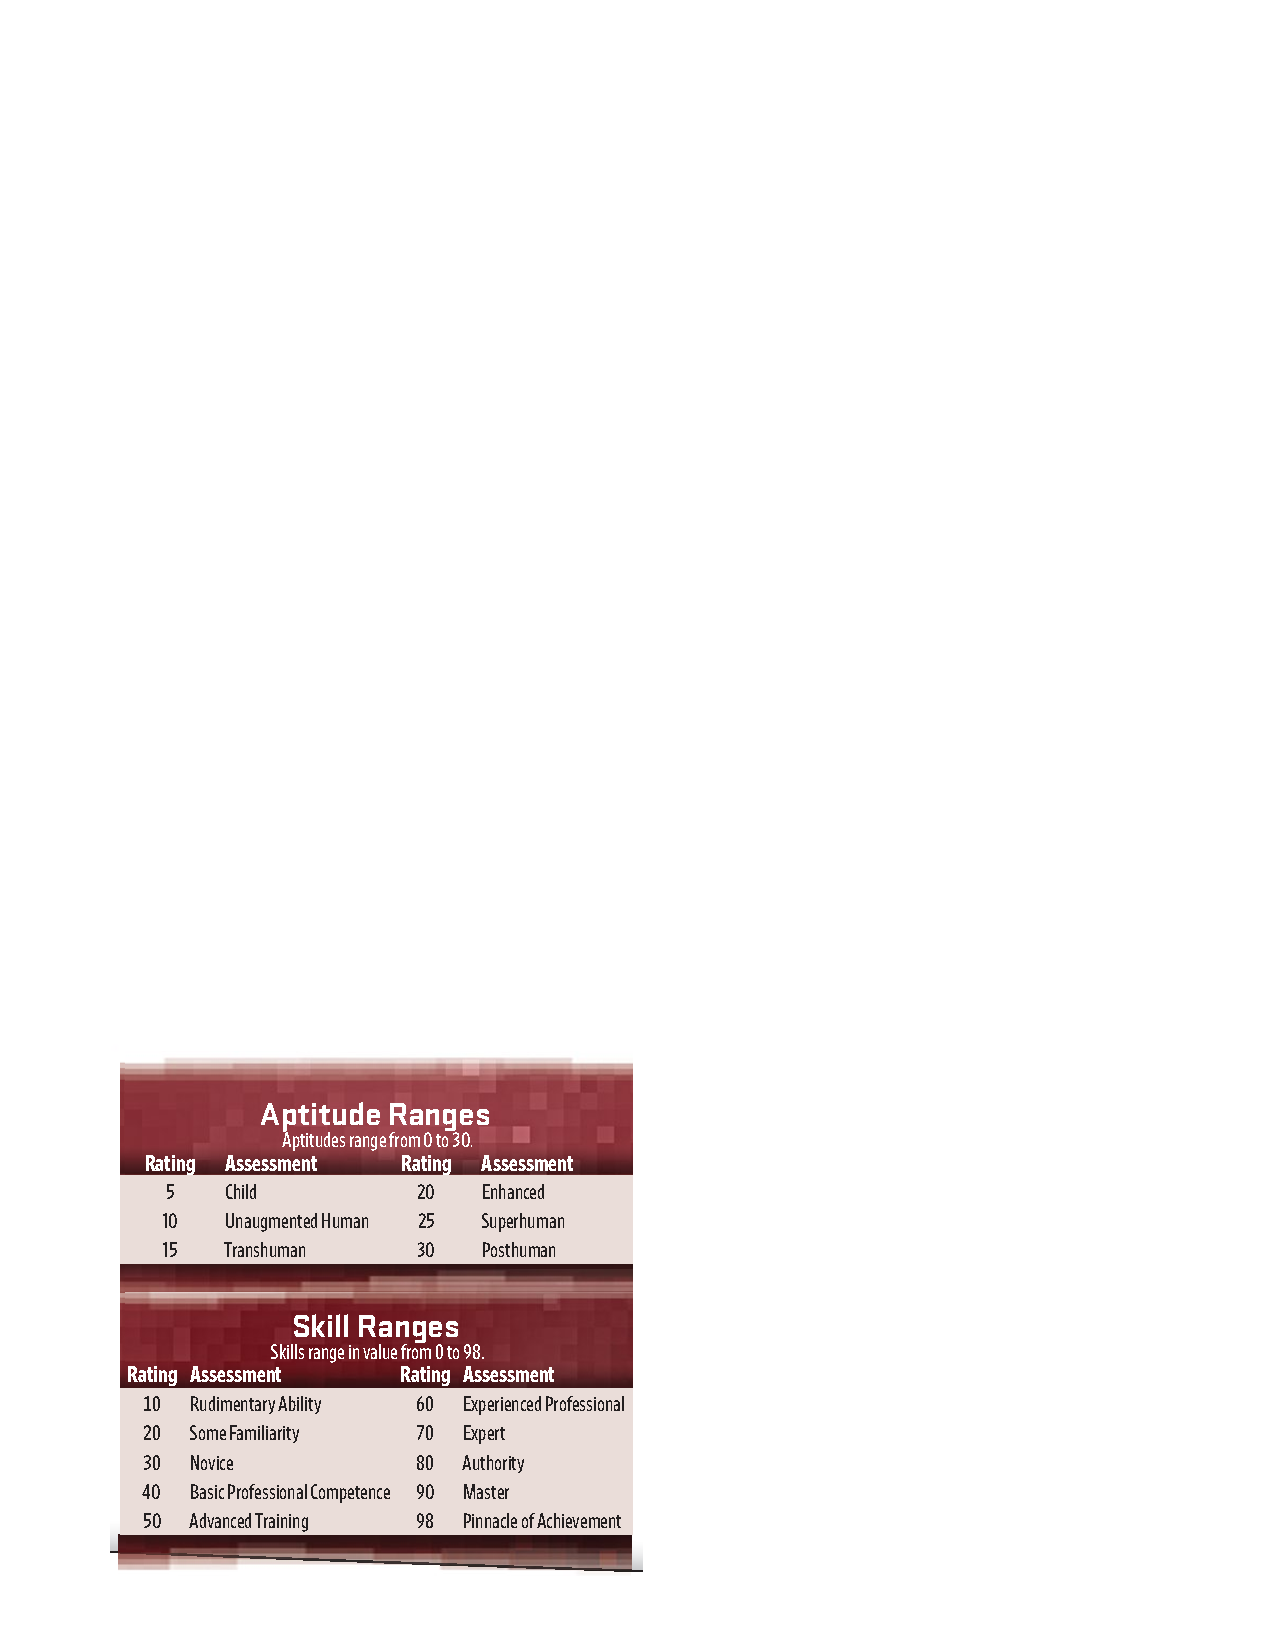
\includegraphics[scale=1.1]{gfx/dice-skills-ranges}%
\end{figure}%

\begin{figure}[htb!]%
   \centering
   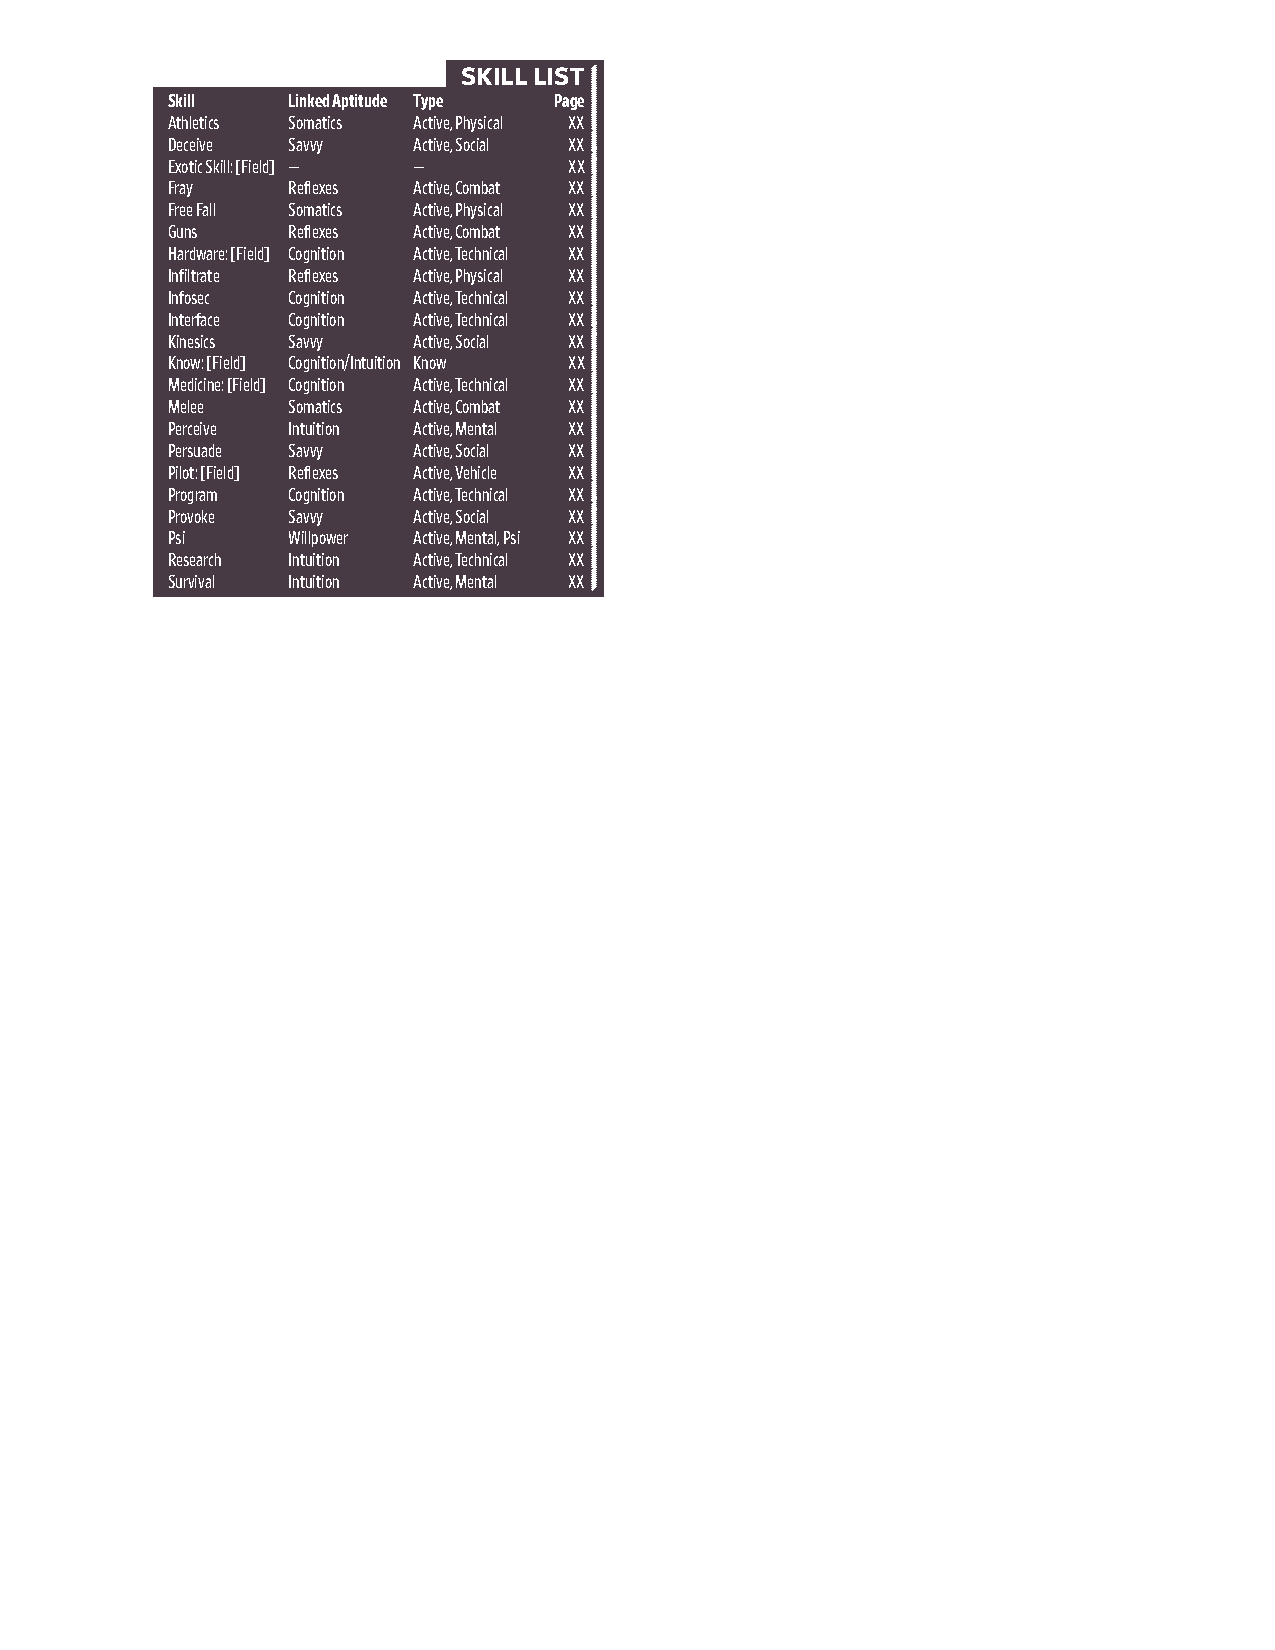
\includegraphics[scale=1.3]{gfx/dice-skills}%
\end{figure}%




\begin{eptable}{ l | X }
   \epheader{2}{Complementary Know Skills}
   \num{40} - \num{59} & Modifier \modifier{+10} for active skill.\\
   \num{60} - \num{79} & Modifier \modifier{+20} for active skill.\\
   \num{80}+ &  Modifier \modifier{+30} for active skill.\\
\end{eptable}


\begin{itemize}
 \itembox Complementary skill bonuses are granted if an appropriate
    Know skill is used to supplement an Active skill.
  \itembox This \textbf{only} applies if the Active skill does not
    incorporate the knowledge of the Know skill already. For example
    \textit{Know: Religious Cults} when doing \textit{Persuation}.
    But not \textit{Know: Computer Science} when doing \textit{Infosec}.

\end{itemize}
